\clearpage 
%\begin{center}
%	\noindent {\LARGE \textbf{Appendix --- For Online Publication}}
%\end{center}
\section{Appendix Figures and Tables} \label{app:add-figs}


\setcounter{table}{0}
\setcounter{figure}{0}
\setcounter{equation}{0}	
\renewcommand{\thetable}{A\arabic{table}}
\renewcommand{\thefigure}{A\arabic{figure}}
\renewcommand{\theequation}{A\arabic{equation}}


\begin{figure}[htp]
	\caption{Distribution of the last digits of new hires' contracted salaries} \label{fig_last_digits}
	\centering
	\begin{subfigure}[t]{.48\textwidth}
		\caption*{Panel A. Last two digits} \label{fig_last_2digits}
		\centering
		\includegraphics[width=\textwidth]{../results/fig_last_2dig}
	\end{subfigure}
	\hfill        
	\begin{subfigure}[t]{0.48\textwidth}
		\caption*{Panel B. Last three digits} \label{fig_last_3digits}
		\centering
		\includegraphics[width=\textwidth]{../results/fig_last_3dig}
	\end{subfigure}		
	\footnotesize \singlespacing \justify \textit{Notes:} Panel A shows the distribution of the last two digits of contracted earnings (in R\$1 bins) in the new-hires sample. Panel B shows the distribution of the last three digits (conditional on the salary having more than three digits).
\end{figure}



\clearpage
\begin{figure}[H]
	\caption{Distribution of monthly earnings in four Brazilian datasets}\label{fig_bunching_data}
	\centering
	\begin{subfigure}[t]{.48\textwidth}
		\caption*{Panel A. Household Survey (PNAD)}\label{fig_bunching_pnad}
		\centering
		\includegraphics[width=\linewidth]{../results/fig_1bins_pnad}
	\end{subfigure}
	\hfill		
	\begin{subfigure}[t]{0.48\textwidth}
		\caption*{Panel B. Labor Force Survey (PME)}\label{fig_bunching_pme}
		\centering
		\includegraphics[width=\linewidth]{../results/fig_1bins_pme}
	\end{subfigure}
	\hfill		
	\begin{subfigure}[t]{.48\textwidth}
		\caption*{Panel C. Population Census}\label{fig_bunching_cen}
		\centering
		\includegraphics[width=\linewidth]{../results/fig_1bins_cen}
	\end{subfigure}
	\hfill		
	\begin{subfigure}[t]{0.48\textwidth}
		\caption*{Panel D. Social Programs Registry}\label{fig_bunching_cad}
		\centering
		\includegraphics[width=\linewidth]{../results/fig_1bins_cad}
	\end{subfigure}	
	\includegraphics[width=.9\linewidth]{../results/fig_1bins_leg}
	\hfill				
	{\footnotesize
		\singlespacing \justify
		
		\textit{Notes:} This figure shows the distribution of monthly earnings in the dataset listed in the panel title. The datasets are the 2013 Brazilian Household Survey (\textit{Pesquisa Nacional por Amostra de Domicílios}, abbreviated PNAD), the 2013 Brazilian Labor Force Survey (\textit{Pesquisa Mensal de Emprego}, abbreviated PME), the 2010 Brazilian Population Census (\textit{Censo Demográfico}), and the 2013 Social Programs Registry of Individuals (\textit{Cadastro Único}). I focus on the monthly earnings of full-time employed workers aged 18--65. I exclude workers employed by public-sector firms and individuals who work without remuneration. 
		
	}
\end{figure}



\clearpage
\begin{figure}[H]
	\caption{Histogram of the share of workers hired at a round salary in each firm} \label{fig_hist_bunch_firms}
	\centering
	\begin{subfigure}[t]{.48\textwidth} 
		\caption*{Panel A. All firms \\ ~ }
		\centering
		\includegraphics[width=\textwidth]{../results/fig_shrhires_10} \label{fig_hist_bunch_firms_10}
	\end{subfigure}
	\hfill		
	\begin{subfigure}[t]{0.48\textwidth}
		\caption*{Panel B. Firms that hired five or more workers in the sample}
		\centering
		\includegraphics[width=\textwidth]{../results/fig_shrhires_10_p5hires} \label{fig_hist_bunch_firms_10_5hires}
	\end{subfigure}	
	\footnotesize \singlespacing \justify \textit{Notes:} This figure show histograms of the share of workers in each firm hired at a round-numbered salary in the firm random sample. Panel A shows the histogram for all firms. Panel B shows the histogram for the subset of firms that hired at least five workers during 2003--2017.
\end{figure}	


\clearpage
\begin{figure}[H]
	\caption{Compensation report for an economist in Ithaca, NY, USA}\label{fig_payscale}
	\centering
	\vspace{.5cm}
	
	\begin{subfigure}[t]{1\textwidth}
		\caption*{Panel A. Factors that affect the compensation report}
		\centering
		\includegraphics[width=\textwidth]{../results/fig_payscale_factors}
	\end{subfigure} \vspace{.7cm}
	
	\begin{subfigure}[t]{0.7\textwidth}
		\caption*{Panel B. Suggested compensation}
		\centering
		\includegraphics[width=\textwidth]{../results/fig_payscale_comp_report} 
	\end{subfigure}
	\footnotesize \singlespacing \justify \textit{Notes:} This figure shows a compensation report provided by the firm PayScale, based on a query by the author. These compensation reports are advertised as the ``right pay'' for a prospective candidate.
\end{figure}


\clearpage
\begin{figure}[H]
	\caption{Wage compression and wage stickiness in the salaries of large firms' new hires} \label{fig_wage_comp_bigf}
	\centering
	\begin{subfigure}[t]{.48\textwidth}
		\caption*{Panel A. Outcome: Gini coefficient}
		\centering
				\includegraphics[width=\linewidth]{../results/fig_wage_comp_gini_bigf}
	\end{subfigure}
	\hfill		
	\begin{subfigure}[t]{0.48\textwidth}
		\caption*{Panel B. Outcome: Percentiles ratios}
		\centering
				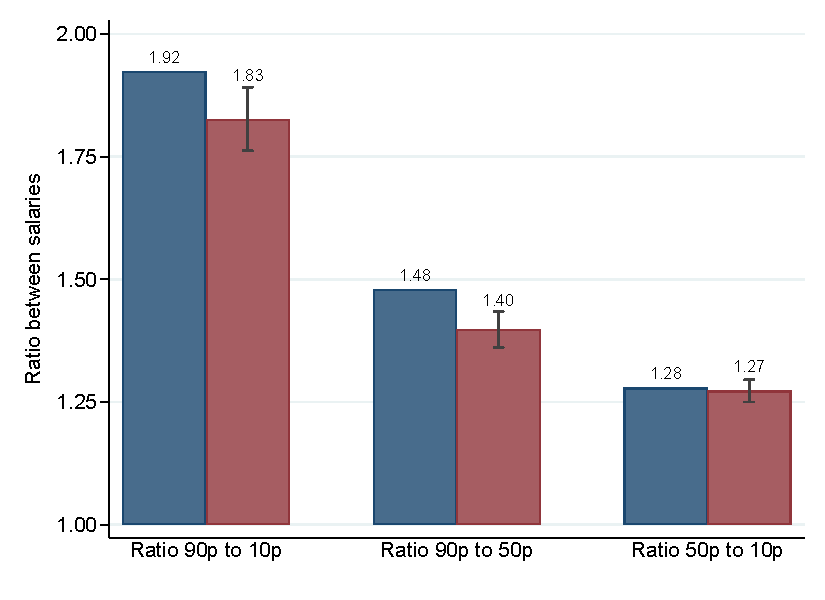
\includegraphics[width=\linewidth]{../results/fig_wage_comp_ratios_bigf}
	\end{subfigure}
	\centering	
	\begin{subfigure}[t]{0.48\textwidth}
		\centering	
		\caption*{Panel C. Outcome: Initial wage remained constant in nominal terms ratios}
		\centering
				\includegraphics[width=\linewidth]{../results/fig_wage_sticky_bigf}
	\end{subfigure}
	
	\vspace{-.3cm}
	
	\begin{subfigure}[t]{\textwidth}		
		\centering
				\includegraphics[width=0.75\linewidth]{../results/fig_wage_comp_leg}
	\end{subfigure}
	\hfill \vspace{-.5cm}	
	{\footnotesize
		\singlespacing \justify
		
		\textit{Notes:} This figure is analogous to Figure \ref{fig_wage_comp}, but the estimates are conditional on firms who, on average across all years in the sample, employ more than five workers. See the notes to Figure \ref{fig_wage_comp} for details on how the figure is constructed, the set of control variables, the definition of the dependent variables, and sample restrictions.
		
	}
\end{figure}




\clearpage
%\begin{sidewaystable}
\begin{table}[H]{\footnotesize
		\begin{center}
			\caption{The characteristics of bunching firms} \label{reg_firm_char}
			\newcommand\w{1.55}
			\begin{tabular}{l@{}lR{\w cm}@{}L{0cm}R{\w cm}@{}L{0cm}R{\w cm}@{}L{0.5cm}R{\w cm}@{}L{0cm}R{\w cm}@{}L{0cm}R{\w cm}@{}L{0.5cm}}
				\midrule
				&& \multicolumn{6}{c}{All firms} & \multicolumn{6}{c}{Large firms} \\ \cmidrule{3-7} \cmidrule{9-14}
				
				&& Bunching  && Non-      && Difference  && Bunching  && Non-         && Difference \\
				&& firms     && bunching  &&             && firms     && bunching      &&              \\
				&& (1) && (2)            && (3) && (4) && (5) && (6)  \\
				\midrule
				
				\ExpandableInput{../results/char_lhiring_exp} 
				\ExpandableInput{../results/char_lmean_size} 
				\ExpandableInput{../results/char_firm_age} 
				\ExpandableInput{../results/char_has_hr} 
				\ExpandableInput{../results/char_ceo_edu} 
				\ExpandableInput{../results/char_lmean_pay} 
				\midrule
				%				\ExpandableInput{char_n} 
				%				\midrule
			\end{tabular}
		\end{center}
		\begin{singlespace}  \vspace{-.5cm}
			\noindent \justify \textit{Notes:} This table shows average firm characteristics of bunching firms and non-bunching firms. Bunching firms are defined as firms that hired all new hires at a round-numbered salary in the sample. Large firms are those who employ, on average across all years, more than five workers in the sample. Heteroskedasticity-robust standard errors clustered at the firm level in parentheses. $^{***}$, $^{**}$ and $^*$ denote significance at the 1\%, 5\% and 10\% levels.
			
		\end{singlespace} 	
	}
\end{table}
%\end{sidewaystable}




\clearpage 
\begin{table}[H]{\footnotesize
		\begin{center}
			\caption{Robustness of market outcomes regressions to excluding small firms} \label{reg_firm_performance_size}
			\newcommand\w{2.5}
			\begin{tabular}{l@{}lR{\w cm}@{}L{0.45cm}R{\w cm}@{}L{0.45cm}R{\w cm}@{}L{0.45cm}R{\w cm}@{}L{0.45cm}R{\w cm}@{}L{0.45cm}}
				\midrule
				&& New hire  && New hire  && Firm job && Firm left  \\
				&& separated && resigned  && growth rate && market \\
				&& (1) && (2) && (3) && (4) \\
				\midrule
				\ExpandableInput{../results/perf_bunch_bigf} \midrule
				
			\end{tabular}
		\end{center}
		\begin{singlespace}  \vspace{-.5cm}
			\noindent \justify \textit{Notes:} This table displays estimates of $\beta$ from equation \eqref{reg:firm-outcomes}, estimated on the subset of firms that employ, on average across years, more than five workers. See notes to Table \ref{reg_firm_performance} for the list of controls and variable definitions. Heteroskedasticity-robust standard errors clustered at the firm level in parentheses. $^{***}$, $^{**}$ and $^*$ denote significance at the 1\%, 5\% and 10\% levels.
			
		\end{singlespace} 	
	}
\end{table}




\clearpage 
\begin{table}[H]{\footnotesize
		\begin{center}
			\caption{Robustness of market outcomes regressions to controlling for wage level} \label{reg_firm_performance_lev}
			\newcommand\w{2.5}
			\begin{tabular}{l@{}lR{\w cm}@{}L{0.45cm}R{\w cm}@{}L{0.45cm}R{\w cm}@{}L{0.45cm}R{\w cm}@{}L{0.45cm}R{\w cm}@{}L{0.45cm}}
				\midrule
				&& New hire  && New hire  && Firm job && Firm left  \\
				&& separated && resigned  && growth rate && market \\
				&& (1) && (2) && (3) && (4) \\
				\midrule
								\ExpandableInput{../results/perf_bunch_allf_full}  \midrule				
			\end{tabular}
		\end{center}
		\begin{singlespace}  \vspace{-.5cm}
			\noindent \justify \textit{Notes:} This table displays estimates of $\beta$ from equation \eqref{reg:firm-outcomes}. All specifications are estimated at the worker level and include the baseline worker-level controls described in the main text. Additionally, the specifications in this table control for the wage level by including wage fixed effects (in R\$100 bins). See notes to Table \ref{reg_firm_performance} for the list of controls and variable definitions. Heteroskedasticity-robust standard errors clustered at the firm level in parentheses. $^{***}$, $^{**}$ and $^*$ denote significance at the 1\%, 5\% and 10\% levels.
			
			
		\end{singlespace} 	
	}
\end{table}


\clearpage
\begin{table}[H]{\footnotesize
		\begin{center}
			\caption{Robustness of market outcomes regressions to alternative definitions of bunching firms} \label{reg_firm_performance_def}
			\newcommand\w{2.5}
			\begin{tabular}{l@{}lR{\w cm}@{}L{0.45cm}R{\w cm}@{}L{0.45cm}R{\w cm}@{}L{0.45cm}R{\w cm}@{}L{0.45cm}R{\w cm}@{}L{0.45cm}}
				\midrule
				&& New hire  && New hire  && Firm job && Firm left  \\
				&& separated && resigned  && growth rate && market \\
				&& (1) && (2) && (3) && (4) \\
				\midrule
				\multicolumn{10}{l}{\hspace{-1em} \textbf{Panel A. Bunching firm equals one if firm hired all workers at a round number (baseline)}}  \\
				\ExpandableInput{../results/perf_bunch_allf}  \midrule
				
				\multicolumn{10}{l}{\hspace{-1em} \textbf{Panel B.  Bunching firm equals one if firm hired all workers at salaries divisible by 100}}  \\
				\ExpandableInput{../results/perf_bunch100_allf} \midrule
				
				\multicolumn{10}{l}{\hspace{-1em} \textbf{Panel C. Bunching firm equals one if firm hired over 1/2 workers at a round number}}  \\				
				\ExpandableInput{../results/perf_bunch50_allf}  \midrule
				
				\multicolumn{10}{l}{\hspace{-1em} \textbf{Panel D. Bunching firm equals one if firm hired over 2/3 workers at a round number}}  \\
				\ExpandableInput{../results/perf_bunch66_allf}  \midrule
				
				\multicolumn{10}{l}{\hspace{-1em} \textbf{Panel E. Bunching firm dummy defined using \textit{yearly} salaries}}  \\
				\ExpandableInput{../results/perf_bunchyr_allf}  \midrule
			
				
			\end{tabular}
		\end{center}
		\begin{singlespace}  \vspace{-.5cm}
			\noindent \justify \textit{Notes:} This table displays estimates of $\beta$ from equation \eqref{reg:firm-outcomes}, using several alternative definitions of bunching firms. See notes to Table \ref{reg_firm_performance} for the list of controls and variable definitions. Heteroskedasticity-robust standard errors clustered at the firm level in parentheses. $^{***}$, $^{**}$ and $^*$ denote significance at the 1\%, 5\% and 10\% levels.
			
		\end{singlespace} 	
	}
\end{table}



\clearpage 
\begin{table}[H]{\footnotesize
		\begin{center}
			\caption{Robustness of coarse pay-setting across decision environments to excluding small firms} \label{reg_salary_increase_size}
			\newcommand\w{1.45}
			\begin{tabular}{l@{}lR{\w cm}@{}L{0.45cm}R{\w cm}@{}L{0.45cm}R{\w cm}@{}L{0.45cm}R{\w cm}@{}L{0.45cm}R{\w cm}@{}L{0.45cm}R{\w cm}@{}L{0.45cm}}
				\midrule
				&& \multicolumn{12}{c}{Dependent variable:} \\ \cmidrule{3-13}
				&& \multicolumn{3}{c}{Salary increase in R\$}  && \multicolumn{3}{c}{Salary increase in \%} && \multicolumn{3}{c}{Either a round} \\
				&& \multicolumn{3}{c}{is a round number}  && \multicolumn{3}{c}{is an integer} && \multicolumn{3}{c}{number or an integer} & \\
				\cmidrule{3-5} \cmidrule{7-9} \cmidrule{11-13}
				&& (1) && (2) && (3) && (4) && (5) && (6) \\
				\midrule
				\ExpandableInput{../results/heurist_bunch_bigf} 
				Excl. zero growth && No && Yes && No && Yes && No && Yes \\ \midrule 
			\end{tabular}
		\end{center}
		\begin{singlespace}  \vspace{-.5cm}
			\noindent \justify \textit{Notes:} This table displays estimates of $\beta$ from equation \eqref{reg:firm-outcomes}, estimated on the subset of firms that employ, on average across years, more than five workers. Even columns exclude new hires whose salary did not change in nominal terms. See notes to Table \ref{reg_salary_increase} for the list of controls and variable definitions. Heteroskedasticity-robust standard errors clustered at the firm level in parentheses. $^{***}$, $^{**}$ and $^*$ denote significance at the 1\%, 5\% and 10\% levels.
				
			
		\end{singlespace} 	
	}
\end{table}






\clearpage 
\begin{table}[H]{\footnotesize
		\begin{center}
			\caption{Robustness of coarse pay-setting across decision environments to controlling for wage level} \label{reg_salary_increase_lev}
			\newcommand\w{1.45}
			\begin{tabular}{l@{}lR{\w cm}@{}L{0.45cm}R{\w cm}@{}L{0.45cm}R{\w cm}@{}L{0.45cm}R{\w cm}@{}L{0.45cm}R{\w cm}@{}L{0.45cm}R{\w cm}@{}L{0.45cm}}
				\midrule
				&& \multicolumn{3}{c}{Salary increase in R\$}  && \multicolumn{3}{c}{Salary increase in \%} && \multicolumn{3}{c}{Either a round} \\
				&& \multicolumn{3}{c}{is a round number}  && \multicolumn{3}{c}{is an integer} && \multicolumn{3}{c}{number or an integer} & \\
				\cmidrule{3-5} \cmidrule{7-9} \cmidrule{11-13}
				&& (1) && (2) && (3) && (4) && (5) && (6) \\
				\midrule
				\ExpandableInput{../results/heurist_bunch_allf_full} 			
				Excl. zero growth && No && Yes && No && Yes && No && Yes \\ \midrule 			
			\end{tabular}
		\end{center}
		\begin{singlespace}  \vspace{-.5cm}
			\noindent \justify \textit{Notes:} This table displays estimates of $\beta$ from equation \eqref{reg:firm-outcomes}. In addition to the baseline controls, the specifications in this table control for the wage level by including wage fixed effects (in R\$100 bins). Even columns exclude new hires whose salary did not change in nominal terms. See notes to Table \ref{reg_salary_increase} for the list of controls and variable definitions. Heteroskedasticity-robust standard errors clustered at the firm level in parentheses. $^{***}$, $^{**}$ and $^*$ denote significance at the 1\%, 5\% and 10\% levels.
			
		\end{singlespace} 	
	}
\end{table}




\clearpage
\begin{table}[H]{\footnotesize
		\begin{center}
			\caption{Robustness of coarse pay-setting across decision environments to alternative definitions of bunching firms} \label{reg_salary_increase_def}
			\newcommand\w{1.5}
			\begin{tabular}{l@{}lR{\w cm}@{}L{0.45cm}R{\w cm}@{}L{0.45cm}R{\w cm}@{}L{0.45cm}R{\w cm}@{}L{0.45cm}R{\w cm}@{}L{0.45cm}R{\w cm}@{}L{0.45cm}}
				\midrule
				&& \multicolumn{3}{c}{Salary increase in R\$}  && \multicolumn{3}{c}{Salary increase in \%} && \multicolumn{3}{c}{Either a round} \\
				&& \multicolumn{3}{c}{is a round number}  && \multicolumn{3}{c}{is an integer} && \multicolumn{3}{c}{number or an integer} & \\
				\cmidrule{3-5} \cmidrule{7-9} \cmidrule{11-13}
				&& (1) && (2) && (3) && (4) && (5) && (6) \\
				\midrule
				\multicolumn{14}{l}{\hspace{-1em} \textbf{Panel A. Bunching firm equals one if firm hired all workers at a round number (baseline)}}  \\
				\ExpandableInput{../results/heurist_bunch_allf}  \midrule
				
				\multicolumn{14}{l}{\hspace{-1em} \textbf{Panel B.  Bunching firm equals one if firm hired all workers at salaries divisible by 100}}  \\
				\ExpandableInput{../results/heurist_bunch100_allf} \midrule
				
				\multicolumn{14}{l}{\hspace{-1em} \textbf{Panel C. Bunching firm equals one if firm hired over 1/2 workers at a round number}}  \\
				\ExpandableInput{../results/heurist_bunch50_allf}  \midrule
				
				\multicolumn{14}{l}{\hspace{-1em} \textbf{Panel D. Bunching firm equals one if firm hired over 2/3 workers at a round number}}  \\
				\ExpandableInput{../results/heurist_bunch66_allf}  \midrule
				
				\multicolumn{14}{l}{\hspace{-1em} \textbf{Panel E. Bunching firm dummy defined using \textit{yearly} salaries}}  \\
				\ExpandableInput{../results/heurist_bunchyr_allf}  \midrule
				
				Excl. zero growth && No && Yes && No && Yes && No && Yes \\ \midrule
			\end{tabular}
		\end{center}
		\begin{singlespace} \vspace{-.5cm}
			\noindent \justify \textit{Notes:} This table displays estimates of $\beta$ from equation \eqref{reg:firm-outcomes}, using alternative definitions of bunching firms. Even columns exclude new hires whose salary did not change in nominal terms. See notes to Table \ref{reg_salary_increase} for the list of controls and variable definitions. Heteroskedasticity-robust standard errors clustered at the firm level in parentheses. $^{***}$, $^{**}$ and $^*$ denote significance at the 1\%, 5\% and 10\% levels.
			
		\end{singlespace}
		
	}
\end{table}




					
\clearpage
\begin{landscape}
	\begin{table}[H]{\footnotesize
		\begin{center}
			\caption{\centering Testing the predictions of the model using alternative measures of coarse salaries} \label{tab_predictions_rob}
			
			\newcommand\w{2}
			\begin{tabular}{l@{}lR{\w cm}@{}L{0.45cm}R{\w cm}@{}L{0.45cm}R{\w cm}@{}L{0.45cm}R{\w cm}@{}L{0.45cm}R{\w cm}@{}L{0.45cm}R{\w cm}@{}L{0.45cm}}
				\midrule
				& \multicolumn{12}{c}{Dependent variable} \\ \cmidrule{3-13} 
				& \multicolumn{6}{c}{Fraction of workers hired} && \multicolumn{6}{c}{Dummy for hiring a worker} \\
				& \multicolumn{6}{c}{through coarse wage-setting $(\hat{\theta} )$} && \multicolumn{6}{c}{at a round number ($\mathbbm{1}\{w_{i} \in R\}$)} \\
				\cmidrule{3-7} \cmidrule{9-14}
								
				&& (1) && (2) && (3) && (4) && (5) && (6) \\ \addlinespace
				
				\ExpandableInput{../results/reg_mult_logcpi_rob}
				\ExpandableInput{../results/reg_mult_lfirm_size_rob}
				\ExpandableInput{../results/reg_mult_lcdf_hiring_rob}				
				\midrule
				
				Measure of coarse salary: && Div. by 10 (baseline) && Div. by 100 \textcolor{white}{~~~~~~~~} && Div. by 1000 \textcolor{white}{~~~~~~~~} && Div. by 10 (baseline) && Div. by 100 \textcolor{white}{~~~~~~~~} && Div. by 1,000 \textcolor{white}{~~~~~~~~}\\ \addlinespace


								
			\end{tabular}
		\end{center}
		\begin{singlespace} \vspace{-.5cm}
			\noindent \justify \textit{Notes:} This table shows linear correlations between the covariate listed in the row header and the outcome listed in the column header using different measures of coarse salaries. Columns 1 and 4 show the results of the baseline specification, using salaries divisible by 10. Columns 2 and 5 use salaries divisible by 100. Columns 3 and 6 use salaries divisible by 1000.
			
			See notes to Table \ref{tab_predictions} for variable definitions and additional details. Heteroskedasticity-robust standard errors clustered at the firm level in parentheses. $^{***}$, $^{**}$ and $^*$ denote significance at the 1\%, 5\% and 10\% levels.
			
		\end{singlespace} 	
	}
\end{table}
\end{landscape}


\clearpage
\begin{table}[H]{\footnotesize
		\begin{center}
			\caption{Wage compression among new hires of bunching firms} \label{reg_wage_compression}
			\newcommand\w{2}
			\begin{tabular}{l@{}lR{\w cm}@{}L{0.45cm}R{\w cm}@{}L{0.45cm}R{\w cm}@{}L{0.45cm}R{\w cm}@{}L{0.45cm}}
				\midrule
				&& && \multicolumn{6}{c}{Ratio of initial salary percentiles:}  \\
				\cmidrule{5-10}    
				&& Gini && 90th to 10th && 90th to 50th && 50th to 10th  \\
				&& (1) && (2) && (3) && (4) \\
				\midrule
				\multicolumn{6}{l}{\hspace{-1em} \textbf{Panel A. All firms}}  \\
				\ExpandableInput{../results/ineq_bunch_allf} \midrule
				\multicolumn{6}{l}{\hspace{-1em} \textbf{Panel B. Firms with more than five workers}} \\
				\ExpandableInput{../results/ineq_bunch_bigf}  \midrule
			\end{tabular}
		\end{center}
		\begin{singlespace} \vspace{-.5cm}
			\noindent \justify \textit{Notes:} This table displays estimates of $\beta$ from equation \eqref{reg:firm-outcomes}. Each column shows the results using a different dependent variable. In column 1, the dependent variable is the Gini coefficient. In column 2, the ratio between the 90th and 10th percentiles of the contracted salary distribution among all the new hires in each firm. In column 3, the ratio between the 90th and the 50th percentiles. In column 4, the ratio between the 50th and 10th percentiles. 
			
			I use the firm random sample to estimate all regressions. The regressions are estimated at the firm-by-year level on firms that hired at least two workers in my sample.
			
			The regressions control for firm age, share of employees with completed high school, share of employees with completed college, educational attainment of the firm manager, a dummy for having an HR department, the mean earnings of the firm employees, firm size fixed effects, number of hires fixed effects, and industry-by-microregion-by-year fixed effects. 
			
			Heteroskedasticity-robust standard errors clustered at the firm level in parentheses. $^{***}$, $^{**}$ and $^*$ denote significance at the 1\%, 5\% and 10\% levels.
			
		\end{singlespace}
	}
\end{table}



